\section{Protection vers le microscope}
Cette section explique les différentes étapes de la conception de la protection vers le microscope, la modélisation de celle-ci, la fabrication des pièces ainsi que le montage final.
\subsection{Réflexion préliminaire}
Contrairement à la précédente protection, la platine bouge dans l'espace sur les trois plans X,Y et Z. Il faut, dans ce cas, trouver un moyen de faire une protection qui puisse être mobile afin de supporter les efforts dans toutes les directions. La platine peut se déplacer d'environ 12~mm en X et Y, et de 25~mm en Z.

La première approche s'est tournée vers de l'impression 3D de plastique souple, tel que du TPU. Ses propriétés élastiques permettent d'avoir une certaine liberté de mouvement.

Les Figures~\ref{zigzag_model}~et~\ref{zigzag_reel} illustrent un modèle 3D de test avec une géométrie en \textit{zigzag}, afin de tester ses propriétés élastiques. Ce modèle n'a pas été concluant, la structure est trop rigide en élasticité. Il faut penser que ce test se base uniquement sur un seul plan, donc si on veut avoir une protection qui se déforme sous les trois plans, ce n'est pas la bonne solution.

\begin{minipage}[c]{0.48\textwidth}
    \begin{center}
        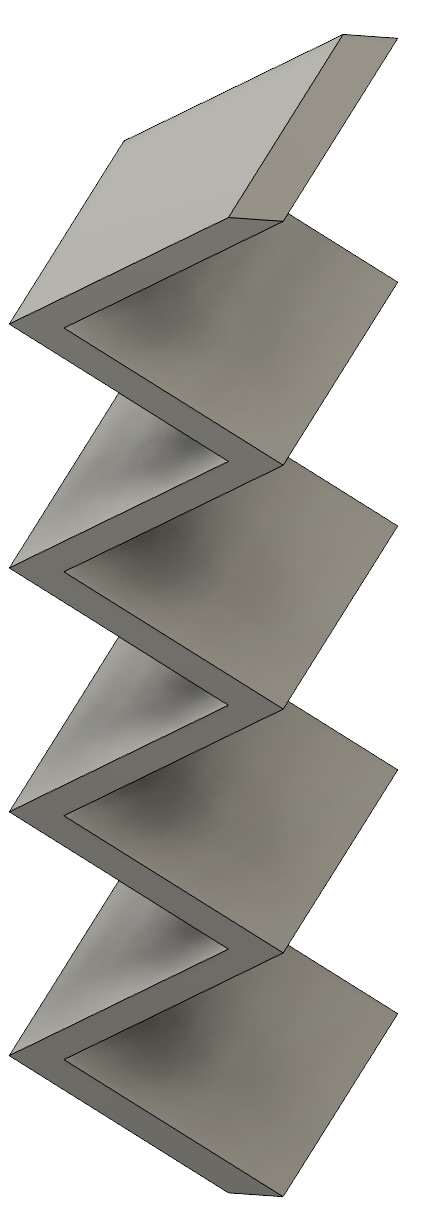
\includegraphics[width=0.2\textwidth]{assets/figures/Protections_laser/Securite_mecanique/Protection_vers_microscope/zigzag_model.jpeg}
    \end{center}
    \captionof{figure}{Modèle 3D avec géométrie en zigzag}
    \label{zigzag_model}
\end{minipage}\hfill
\begin{minipage}[c]{0.48\textwidth}
    \begin{center}
        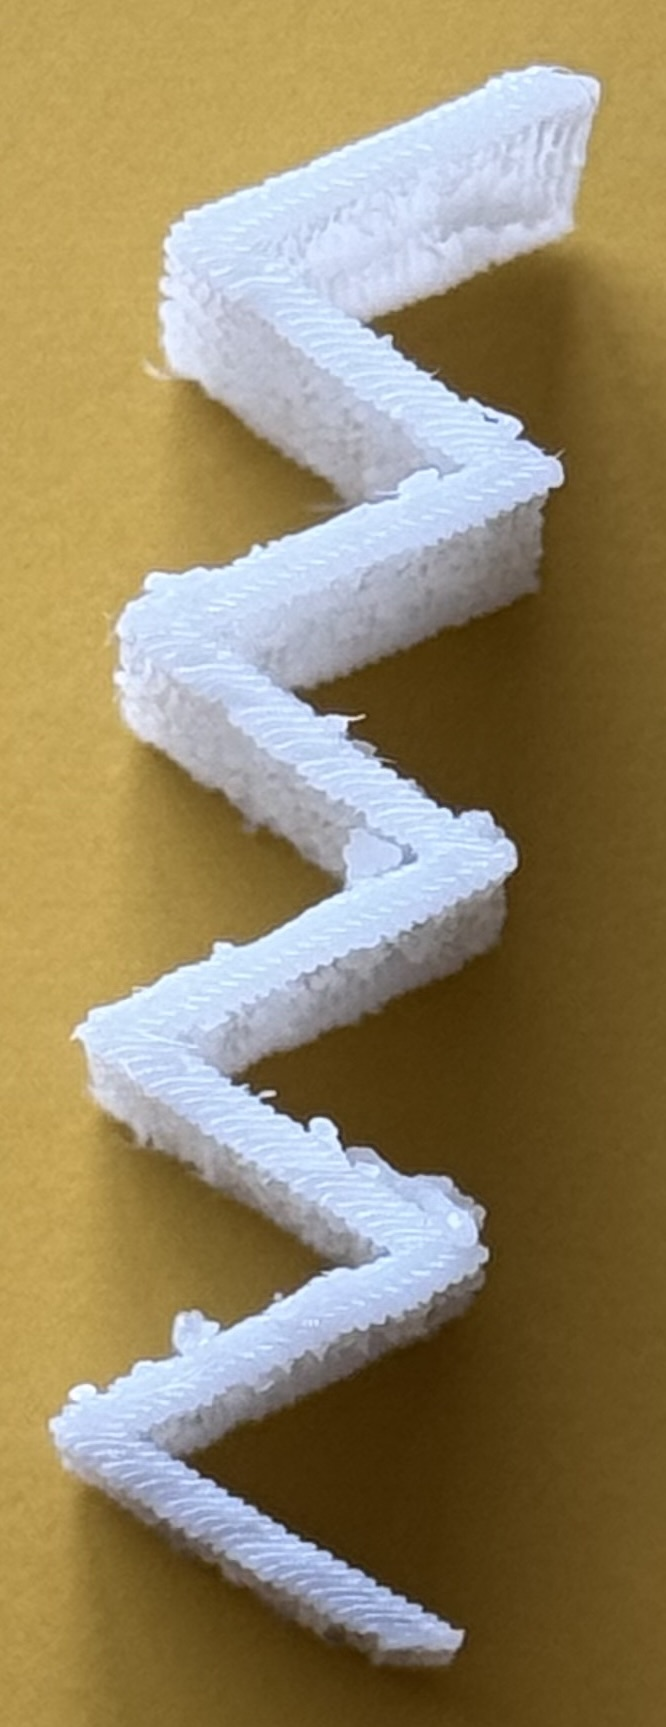
\includegraphics[width=0.2\textwidth]{assets/figures/Protections_laser/Securite_mecanique/Protection_vers_microscope/zigzag_reel.jpeg}
    \end{center}
    \captionof{figure}{Impression 3D en TPU du modèle avec géométrie en zigzag}
    \label{zigzag_reel}
\end{minipage}

La solution retenue pour avoir les mouvements les plus optimaux a été de créer une protection en tissu, associée à des impressions 3D en PLA.

\subsection{Modélisation de la protection}
\begin{minipage}[c]{0.38\textwidth}
    Afin de mieux comprendre les choix de conception et les étapes faites pour réaliser la protection, la Figure~\ref{model_3D_microscope} représente la modélisation complète de la protection vers le microscope. Les modélisations créées pour cette protection sont en couleur sur la représentation 3D.
\end{minipage}\hfill
\begin{minipage}[c]{0.58\textwidth}
    \begin{center}
        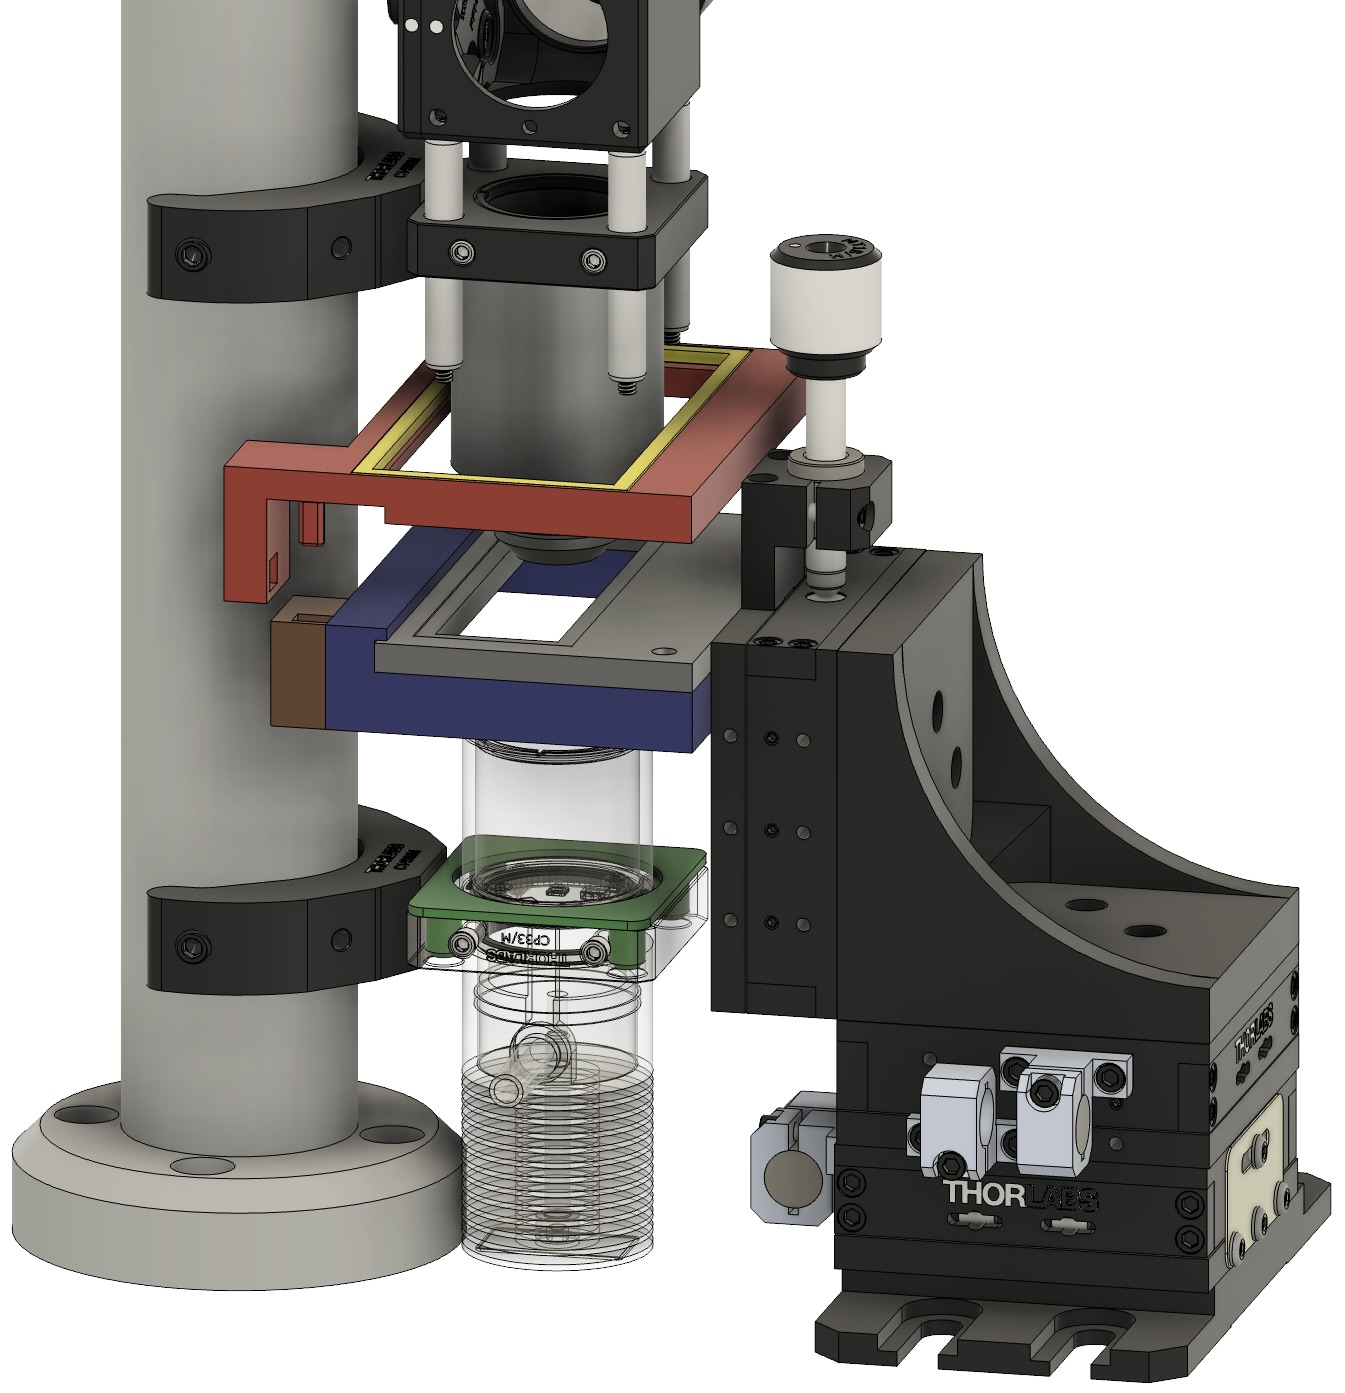
\includegraphics[width=\textwidth]{assets/figures/Protections_laser/Securite_mecanique/Protection_vers_microscope/model_3D.jpeg}
    \end{center}
    \captionof{figure}{Modèle 3D complet de la protection vers le microscope}
    \label{model_3D_microscope}
\end{minipage}

% Prompt ChatGPT pour la création du tableau:
% Fais moi un tableau avec les éléments ci-dessous:

% Partie inférieure:
% - En vert, support pour fixer le tissu inférieur à la LED
% - En bleu foncé, support pour fixer le tissu inférieur à la platine
% Partie supérieure:
% - En rouge, support qui vient se clipser sur la platine
% - En brun, boitier pour fixer le fin de course
% - En jaune, cadre pour fixer le tissu supérieur au support rouge

\begin{table}[H]
    \centering
    \begin{tabular}{|c|l|}
        \hline
        \textbf{Couleur}                         & \textbf{Nom de la pièce}                             \\
        \hline
        \multicolumn{2}{|c|}{\textbf{Partie inférieure}}                                                \\
        \hline
        \textcolor[RGB]{70, 170, 70}{Vert}       & Support pour fixer le tissu inférieur à la LED       \\
        \textcolor[RGB]{30, 50, 150}{Bleu foncé} & Support pour fixer le tissu inférieur à la platine   \\
        \hline
        \multicolumn{2}{|c|}{\textbf{Partie supérieure}}                                                \\
        \hline
        \textcolor[RGB]{170, 50, 50}{Rouge}      & Support clipsable sur la platine                     \\
        \textcolor[RGB]{120, 70, 30}{Brun}       & Boîtier pour fixer le fin de course                  \\
        \textcolor[RGB]{233, 173, 56}{Jaune}     & Cadre pour fixer le tissu supérieur au support rouge \\
        \hline
    \end{tabular}
    \caption{Nomenclature des pièces modélisées avec code couleur pour la protection vers le microscope. \cite{chatgptTableProtectionVersMicroscope}}
    \label{tab:nomenclature_pieces_microscope}
\end{table}

\subsubsection{Partie inférieure}
\begin{minipage}[c]{0.48\textwidth}
    Pour fixer le tissu à la LED (pièce \textcolor[RGB]{70, 170, 70}{verte} de la Figure~\ref{model_3D_microscope}), le support montré sur la Figure~\ref{support_inf_tissu_LED} a été pensé. La plaque, désignée par la flèche \textcolor{red}{rouge}, est une plaque de cage.

    \vspace{1em}
    Ses quatre trous sont utilisés avec des petites vis sans tête (flèches \textcolor[RGB]{115, 210, 210}{bleues}), afin de permettre sa fixation au support. Le tissu est pincé entre la plaque et le support imprimé.
\end{minipage}\hfill
\begin{minipage}[c]{0.48\textwidth}
    \begin{center}
        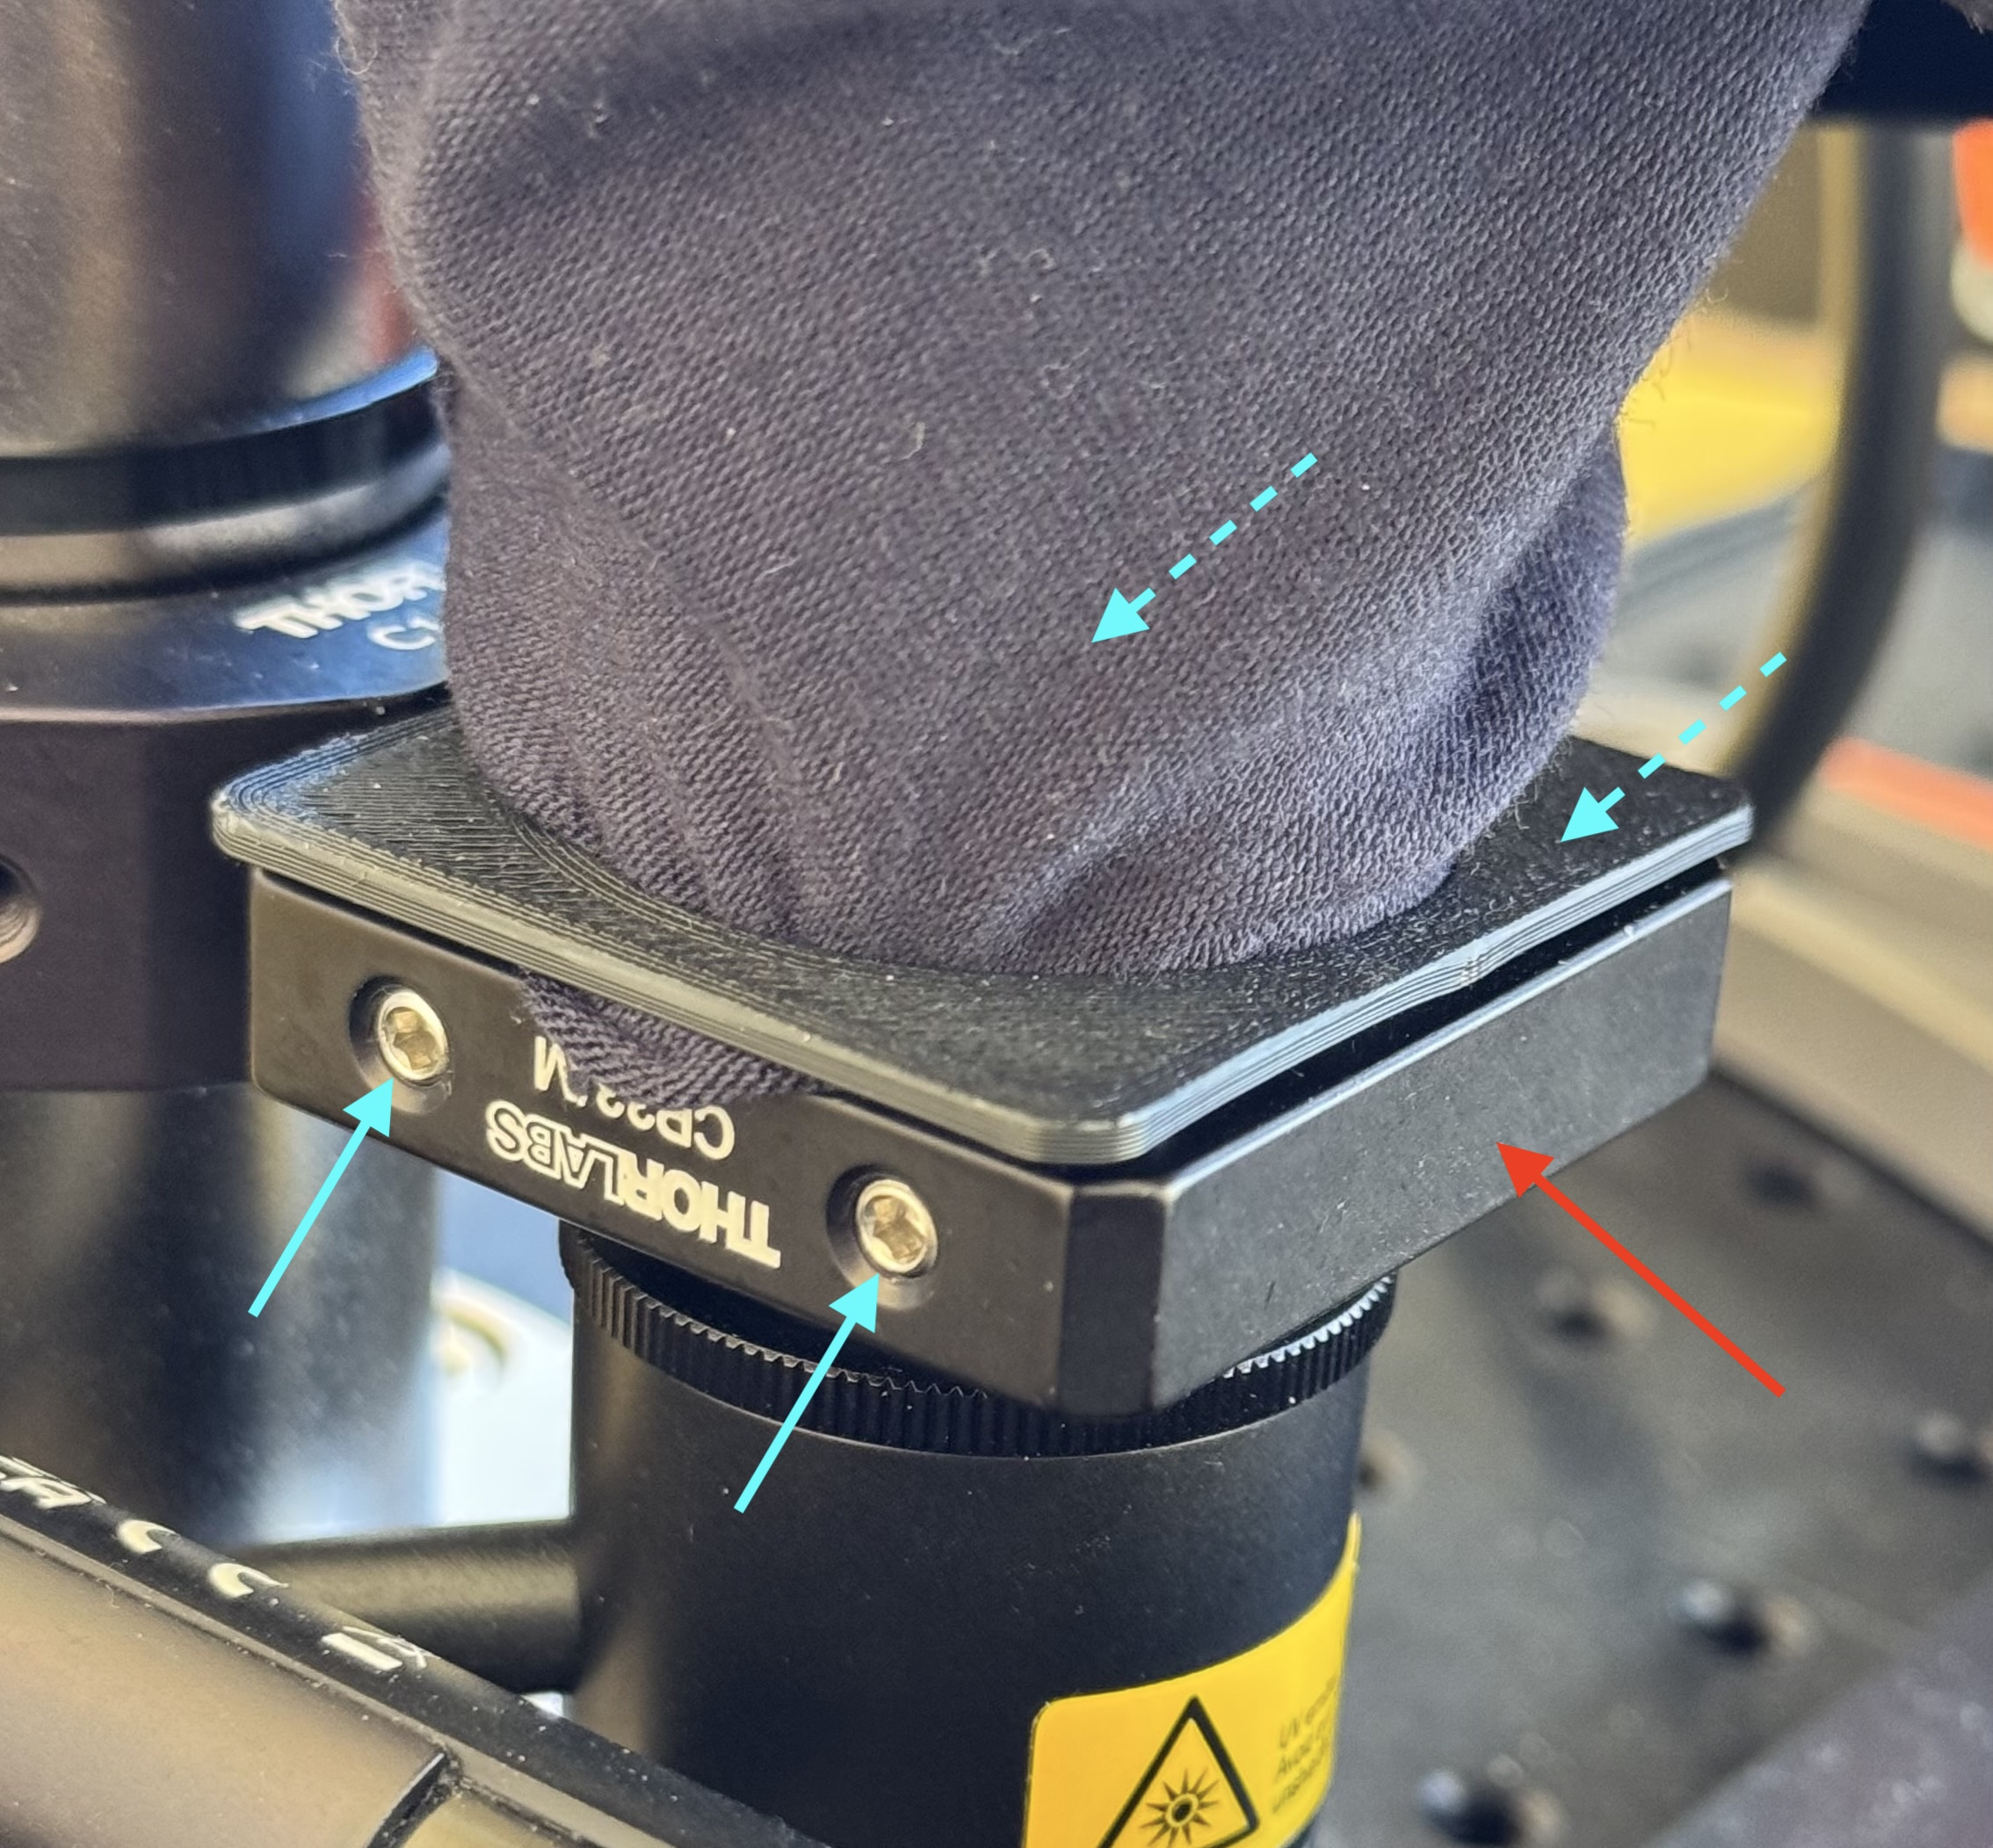
\includegraphics[width=0.9\textwidth]{assets/figures/Protections_laser/Securite_mecanique/Protection_vers_microscope/support_inf_tissu_LED.jpeg}
    \end{center}
    \captionof{figure}{Support pour fixer le tissu inférieur à la LED}
    \label{support_inf_tissu_LED}
\end{minipage}

\begin{minipage}[c]{0.48\textwidth}
    Pour fixer le tissu à la platine (pièce \textcolor[RGB]{30, 50, 150}{bleu foncé} de la Figure~\ref{model_3D_microscope}), le support montré sur la Figure~\ref{support_inf_tissu_platine} (flèche \textcolor{red}{rouge}) a été élaboré.

    \vspace{1em}
    Pour le fixer, les vis montrées par les flèches \textcolor[RGB]{115, 210, 210}{bleues} ont été utilisées. Comme pour la fixation à la LED, ici, le tissu est également coincé entre la platine et le support.
\end{minipage}\hfill
\begin{minipage}[c]{0.48\textwidth}
    \begin{center}
        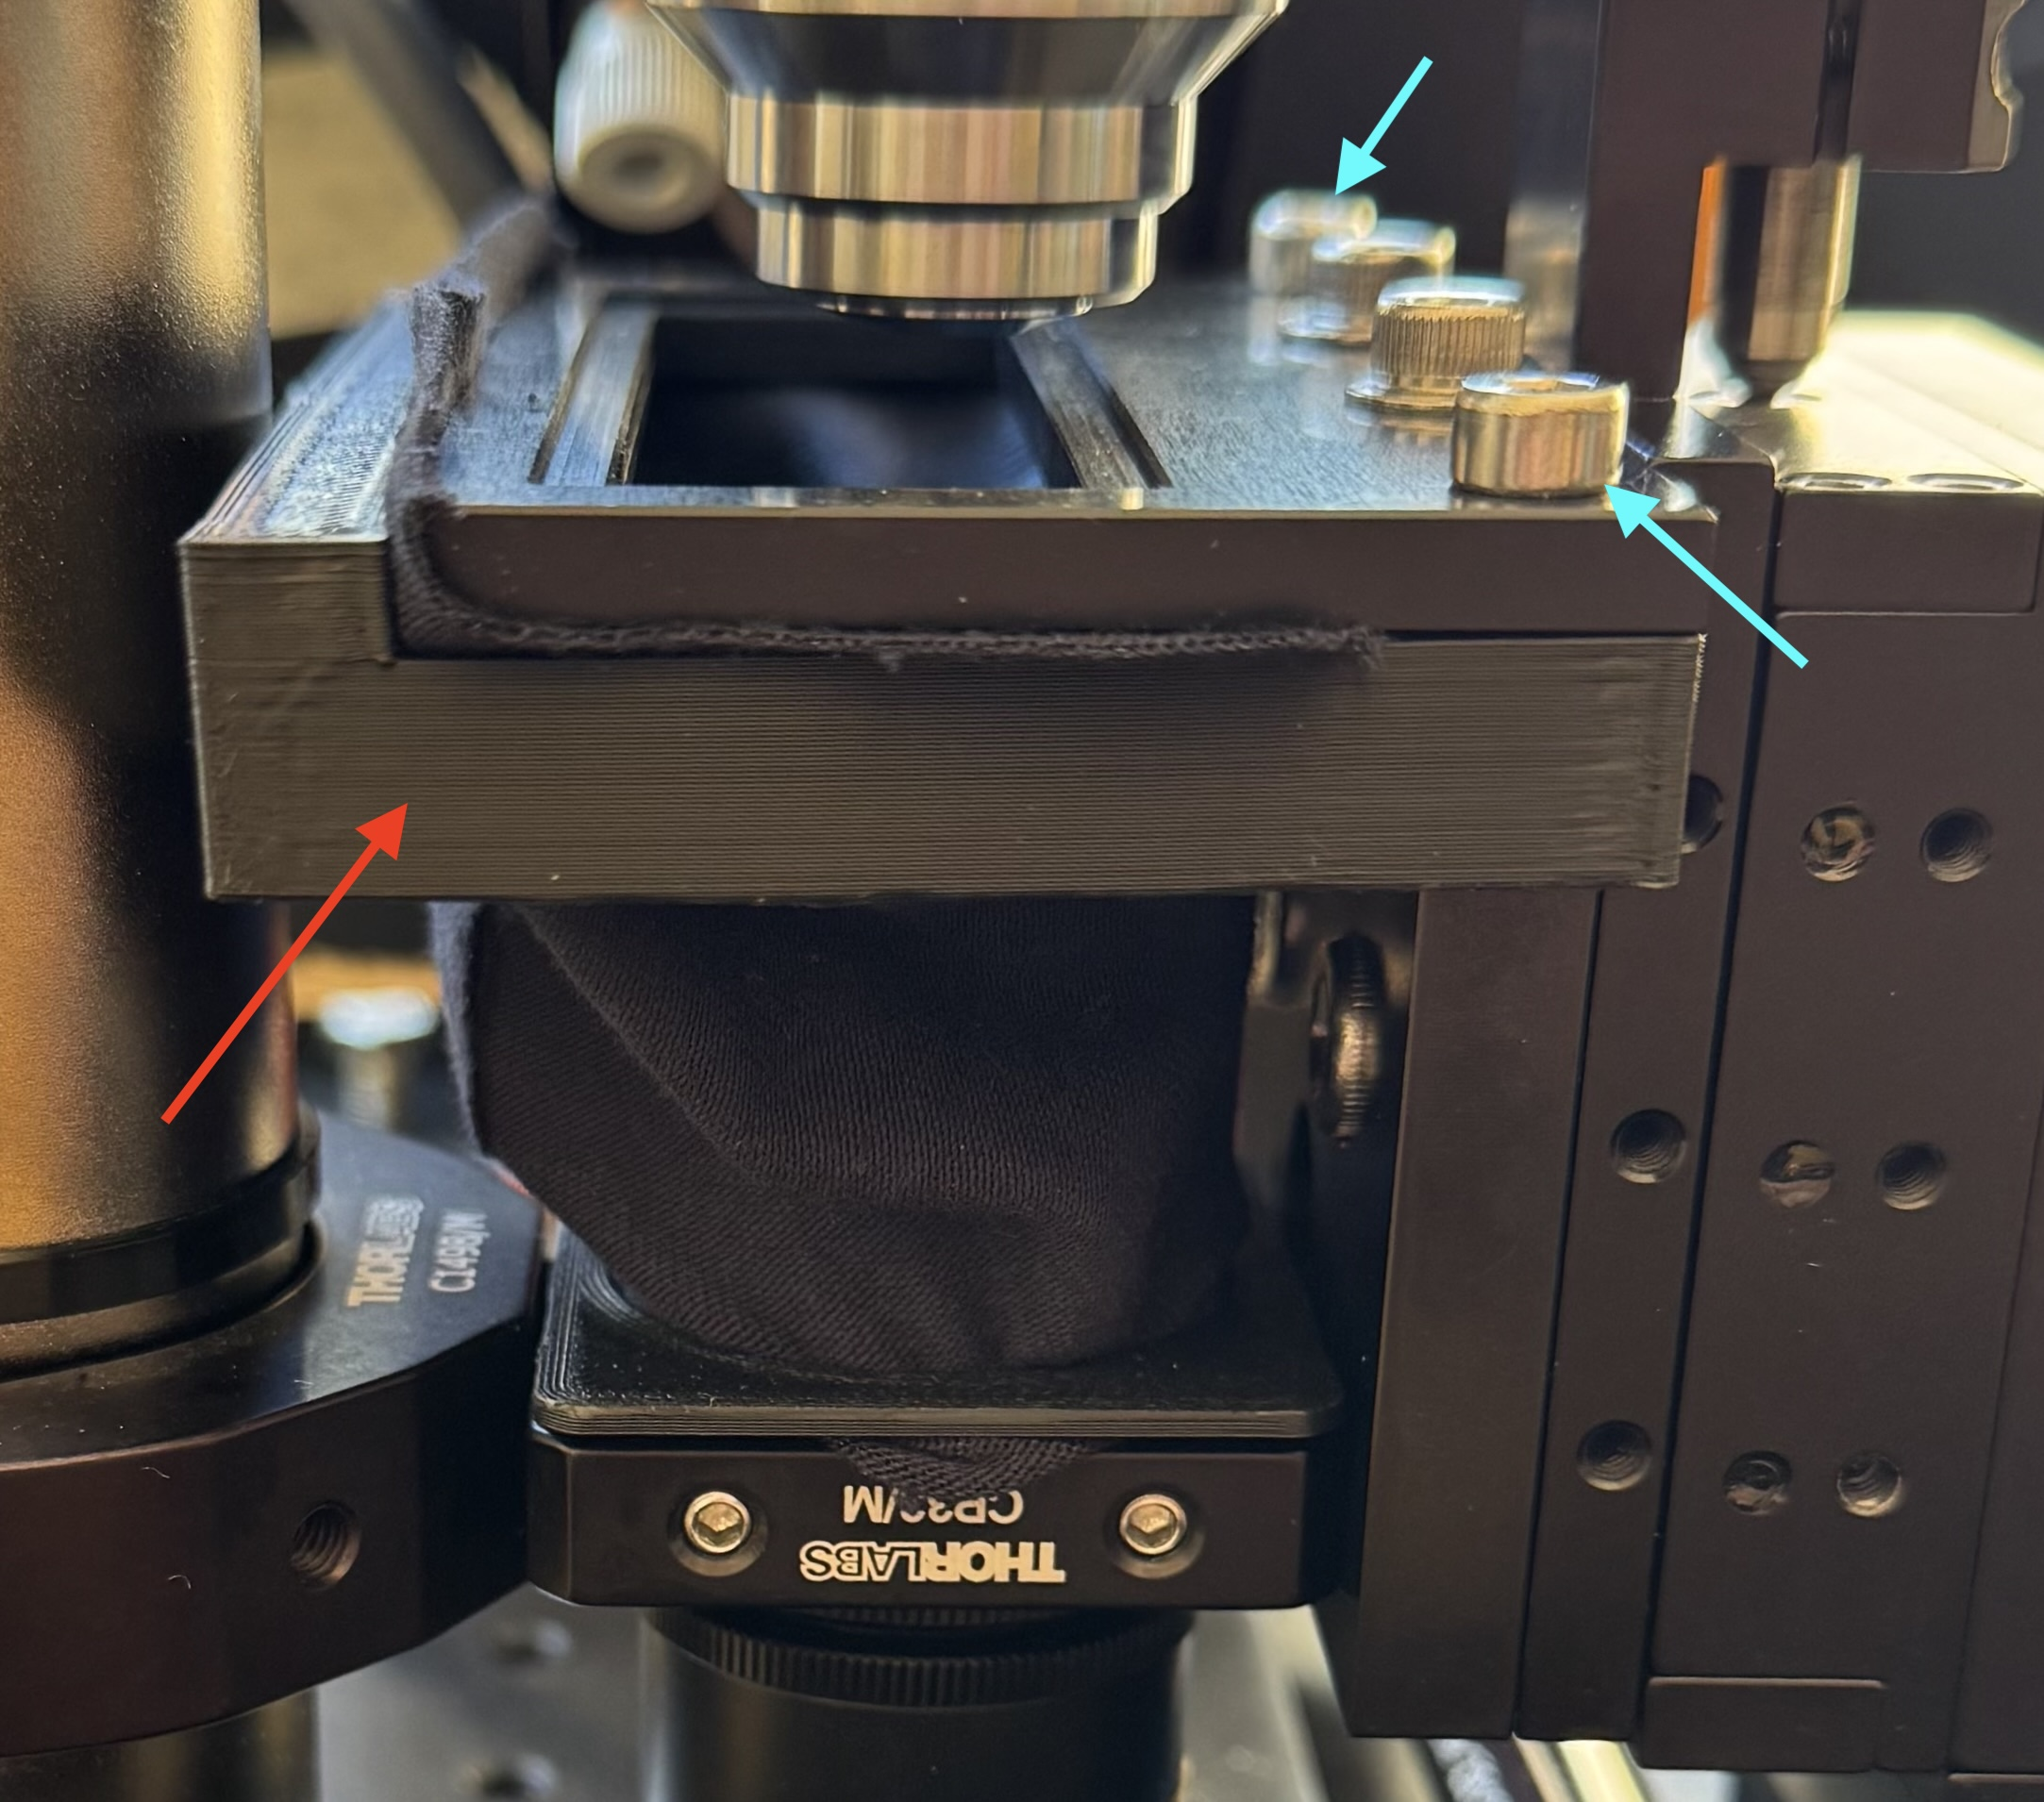
\includegraphics[width=0.9\textwidth]{assets/figures/Protections_laser/Securite_mecanique/Protection_vers_microscope/support_inf_tissu_platine.jpeg}
    \end{center}
    \captionof{figure}{Support pour fixer le tissu inférieur à la platine}
    \label{support_inf_tissu_platine}
\end{minipage}

\subsubsection{Partie supérieure}

\begin{minipage}[c]{0.48\textwidth}
    Pour la partie supérieure, la fixation du tissu est assuré avec le cadre \textcolor[RGB]{233, 173, 56}{jaune} et le support \textcolor[RGB]{170, 50, 50}{rouge} illustré sur la Figure~\ref{model_3D_microscope}. Ce support imprimé est montré par la flèche \textcolor{red}{rouge} sur cette Figure~\ref{support_sup_tissu_microscope}.

    \vspace{1em}
    Pour fixer le tissu à la structure au-dessus du microscope, une attache rapide (flèche \textcolor[RGB]{115, 210, 210}{bleue}) a été utilisé pour le maintenir en place.

\end{minipage}\hfill
\begin{minipage}[c]{0.48\textwidth}
    \begin{center}
        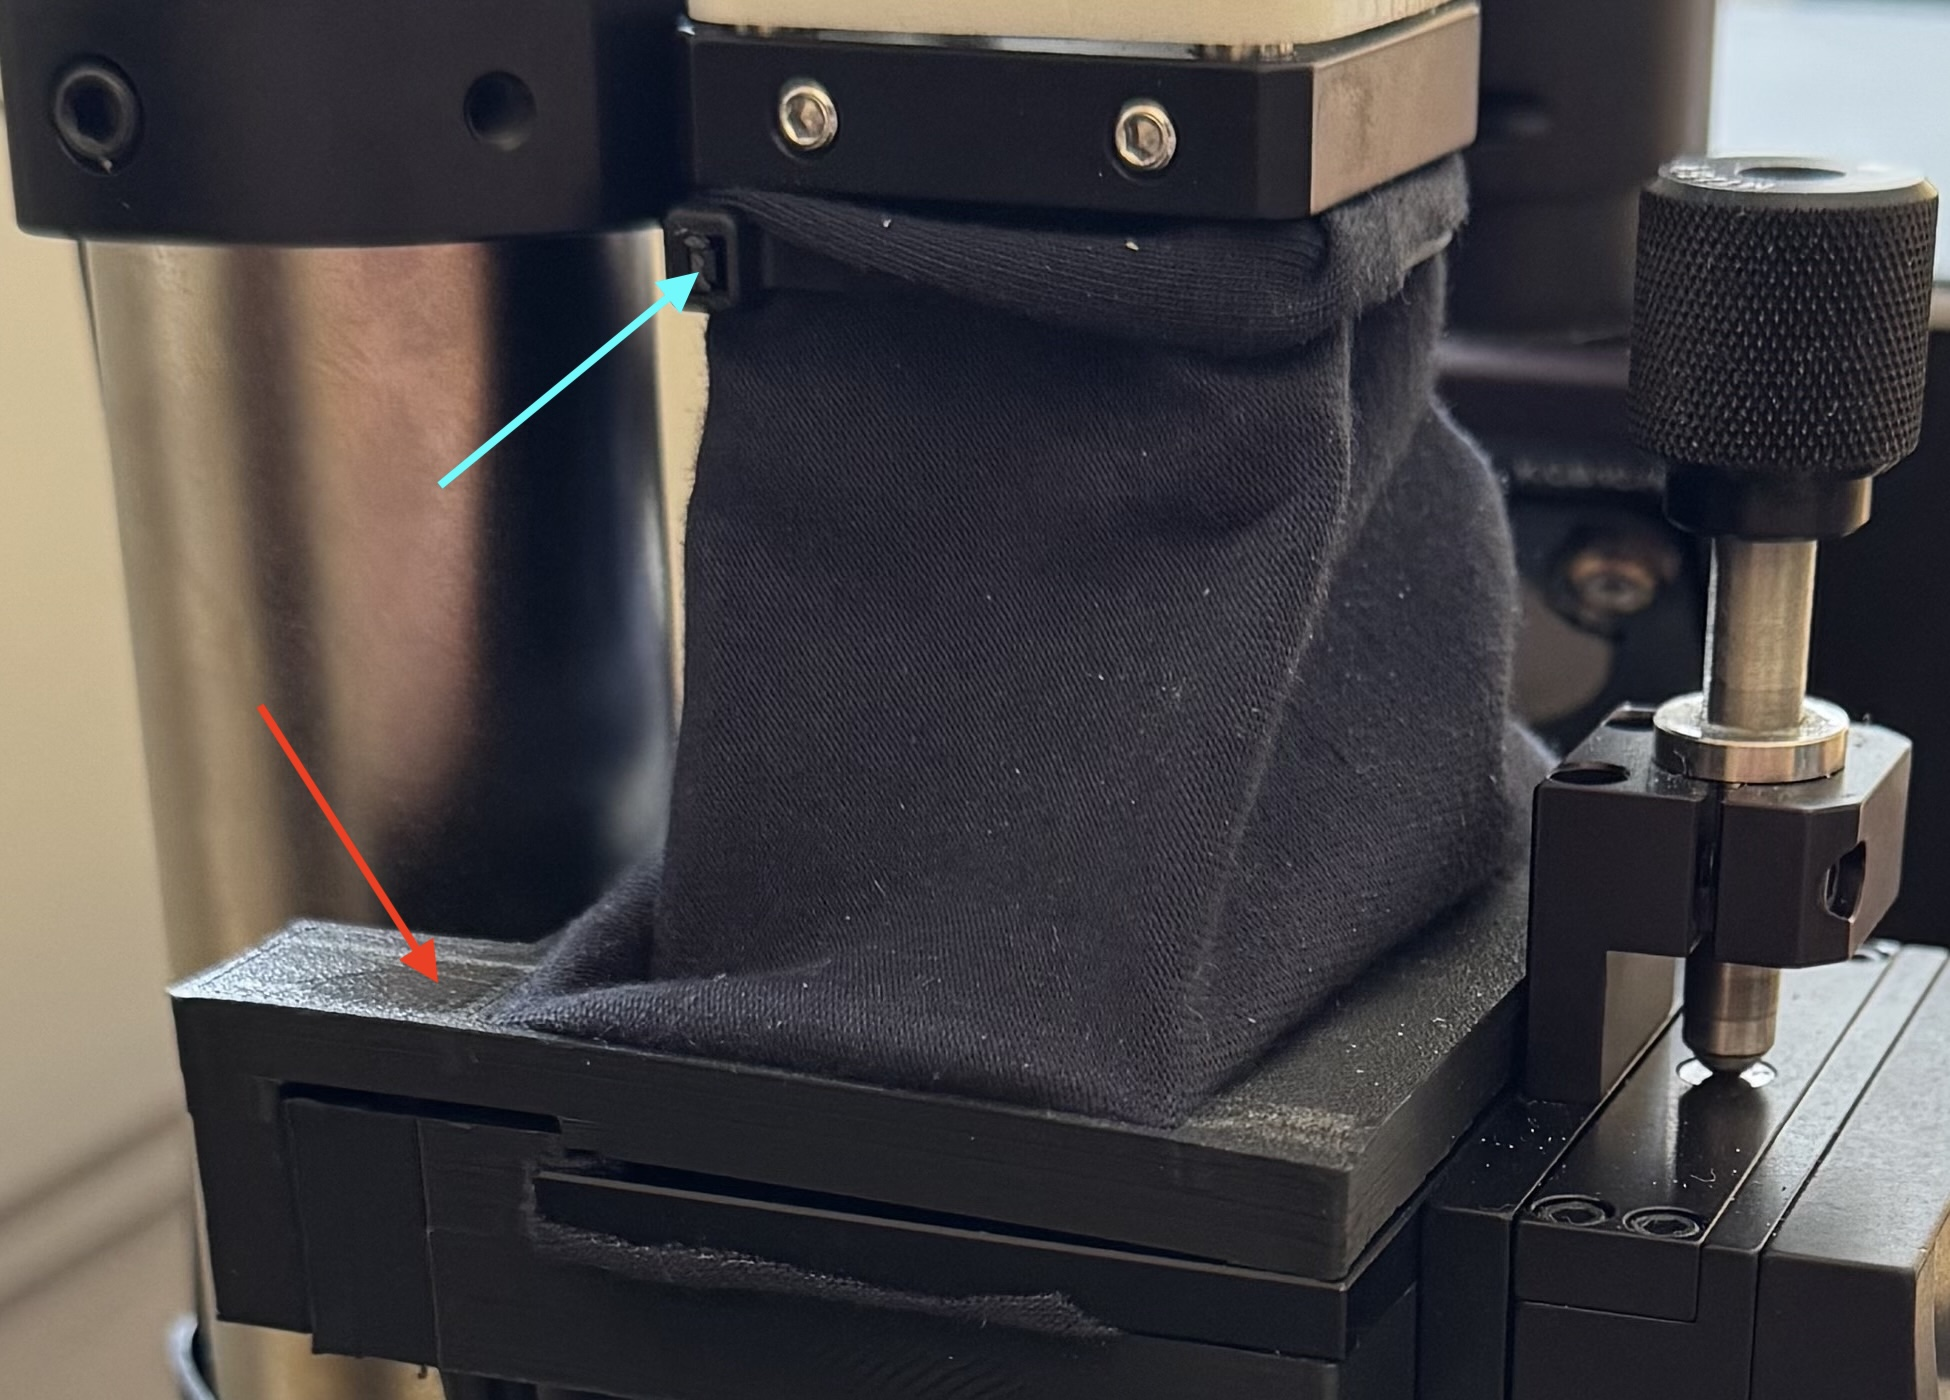
\includegraphics[width=0.9\textwidth]{assets/figures/Protections_laser/Securite_mecanique/Protection_vers_microscope/support_sup_tissu_microscope.jpeg}
    \end{center}
    \captionof{figure}{Support pour fixer le tissu inférieur à la platine}
    \label{support_sup_tissu_microscope}
\end{minipage}

\subsubsection{Fin de course}
\begin{minipage}[c]{0.48\textwidth}
    Afin d'assurer le bon fonctionnement du fin de course, le boîtier modélisé en \textcolor[RGB]{120, 70, 30}{brun} sur la Figure~\ref{model_3D_microscope} a été créé. Son modèle imprimé est représenté par la flèche \textcolor[RGB]{115, 210, 210}{bleue} sur la Figure~\ref{boitier_fin_de_course}.

    \vspace{1em}
    L'axe encadré en \textcolor[RGB]{233, 173, 56}{jaune} assure l'actionnement du fin de course dans le logement du boîtier.

\end{minipage}\hfill
\begin{minipage}[c]{0.48\textwidth}
    \begin{center}
        \includegraphics[width=0.9\textwidth]{assets/figures/Protections_laser/Securite_mecanique/Protection_vers_microscope/boitier_fin_de_course.png}
    \end{center}
    \captionof{figure}{Boîtier pour le fin de course}
    \label{boitier_fin_de_course}
\end{minipage}

\subsection{Points d'améliorations}
\begin{itemize}[label=\textbullet]
    \item Il est possible d'augmenter la sécurité pour cette protection. Même si le fin de course est caché dans son boîtier, il reste possible de l'atteindre avec un objet assez fin. Il faudrait trouver un capteur qui soit presque inviolable comme la charnière de sécurité.
    \item Le montage est minutieux et prend du temps, comparé à la protection à l'entrée du laser.
    \item Un moyen de maintenir ouvert la protection serait plus ergonomique. Actuellement, il faut la tenir soi-même.
    \item Le tissu pourrait être amélioré pour que ce soit plus propre.
    \item La structure manque de solidité, à terme la protection pourrait être usinée dans un matériau plus solide.
\end{itemize}
